\documentclass{article}
\usepackage[utf8]{inputenc}
\usepackage[margin=1in]{geometry}
\usepackage{booktabs}
\usepackage{tabu}
\usepackage[labelfont=bf, skip=5pt, font=small]{caption}
\usepackage[]{subcaption}
\usepackage{graphicx}
\usepackage{fancyhdr}
\usepackage{amsmath}
\usepackage{float} % here for H placement parameter
\usepackage{hyperref}

\font\myfont=cmr12 at 100pt
\title{\Huge DATA304 Project Group 4:\\
  \Huge A study of the LAB cafe at Victoria University}
\author{\Large Kevin Ye, Vivian Dong, Patrick Quito, Tama Hoare }
\date{\Large May 2022}

\begin{document}


\maketitle
\newpage

\section{Introduction}
Suo Lorem ipsum dolor sit amet, consectetur adipiscing elit. Quisque tincidunt justo nec sem aliquet, vel molestie tortor rhoncus. Aliquam scelerisque metus sit amet mattis commodo. Sed tincidunt sapien vitae sapien volutpat, cursus efficitur lacus consequat. Nunc mi dolor, tempor vitae lorem ut, convallis ullamcorper massa. In hendrerit id purus a vulputate. Pellentesque nulla nunc, bibendum quis vulputate sit amet, dictum at nibh. Class aptent taciti sociosqu ad litora torquent per conubia nostra, per inceptos himenaeos. Sed nulla nisi, porttitor porta erat vel, porttitor finibus nisi. Quisque diam diam, egestas id ornare mattis, laoreet vitae justo. Curabitur in nunc ornare, fermentum leo non, hendrerit ipsum. Aliquam erat volutpat. Nunc lobortis sem in orci faucibus suscipit. In hac habitasse platea dictumst. Vivamus ante augue, dictum faucibus efficitur non, consequat non enim.


\noindent Maecenas ullamcorper sem id magna sodales tempor. Sed non est urna. Mauris nec ante quis diam cursus suscipit non imperdiet erat. Donec posuere consectetur hendrerit. Proin pharetra, nulla eu pharetra vulputate, magna mi malesuada enim, non euismod augue lorem quis nunc. Quisque hendrerit euismod hendrerit. Maecenas tempor augue sit amet ultrices elementum. Proin posuere semper diam, ut lobortis sem eleifend sit amet. Nulla ornare eget ligula in ornare. Ut vel finibus ligula. Donec sollicitudin, dolor non porta faucibus, sapien elit ultrices augue, ac mattis ante neque sed neque.

\section{Data analysis}
Phasellus nec lorem nec nibh aliquet imperdiet nec a dolor. Nunc auctor leo sit amet sem suscipit, et accumsan nunc ultrices. Praesent vitae nulla id dolor vulputate porttitor. Integer nisl lorem, dictum nec ultrices at, malesuada sed ligula. Curabitur vehicula orci non libero eleifend commodo. Cras vitae lacus tellus. Nullam feugiat, nisi at tempus rutrum, arcu nibh commodo odio, at aliquet nulla tortor non neque. Nulla eget nulla vel libero suscipit gravida. Conclusion. idskfjslf

\subsection{Fitting best fit distributions (Vivian)}

We tried to approximate "inter-arrival time" and "service time" using the following 12 Distributions: Weibull Minimum Extreme Value distribution, Normal distribution, Weibull Maximum Extreme Value distribution, Beta distribution, Inverse Gaussian distribution, Uniform distribution, Gamma distribution, Exponential distribution, Log-normal distribution, Pearson Type III distribution, Triangular distribution, Erlang distribution. After fitting different distributions, we checked the Goodness of fit based on Chi-square Statistics.\newline

The output for "inter-arrival time" sorted in order of Goodness of fit looks like this:\newline

\begin{table}[h!]
    \centering
    \caption{Distributions listed by Betterment of fit}
    \begin{tabu}{*{2}{X[c]}}
        \toprule
        \textbf{Distribution} & \textbf{chi square}\\
        \midrule
        Pearson Type III distribution & 9.155252\\
        Weibull Minimum Extreme Value distribution & 13.245287\\
        Beta distribution & 21.708357\\
        Log Normal distribution & 25.596288\\
        Inverse Gaussian distribution & 29.389634\\
        Exponential distribution & 29.515278\\
        Gamma distribution & 48.359331\\
        Triangular distribution & 209.930441\\
        Normal distribution & 332.531278\\
        Uniform distribution & 510.690318\\
        Erlang distribution & 672.400334\\
        Weibull Maximum Extreme Value distribution & 1137.915014\\
        \bottomrule
    \end{tabu}
    \label{tab:Inter-arrival Best Fit}
\end{table}

The output for 'service time' sorted in order of Goodness of fit looks like this:\newline

\begin{table}[h!]
    \centering
    \caption{Distributions listed by Betterment of fit}
    \begin{tabu}{*{2}{X[c]}}
        \toprule
        \textbf{Distribution} & \textbf{chi square}\\
        \midrule
        Beta distribution & 1.231338\\
        Weibull Minimum Extreme Value distribution & 2.831316\\
        Pearson Type III distribution & 4.130412\\
        Gamma distribution & 4.131762\\
        Erlang distribution & 4.132443\\
        Inverse Gaussian distribution & 10.560874\\
        Log Normal distribution & 11.688749\\
        Exponential distribution & 29.775131\\
        Triangular distribution & 39.441479\\
        Normal distribution & 140.194689\\
        Uniform distribution & 305.594183\\
        Weibull Maximum Extreme Value distribution & 1080.829277\\
        \bottomrule
    \end{tabu}
    \label{tab:Service Best Fit}
\end{table}

The Chi-square statistics suggest that the Pearson Type III distribution best approximates 'inter-arrival time'. We can also see that Beta distribution is the best fit for 'service time'.\newline

The python code using the Scipy Library to fit the distribution is from here:
\url{https://github.com/mungoliabhishek/Distribution-Fitting-Used_Car_Dataset/blob/master/Workbook.ipynb}\newline

Suppose we had more time to do this part. In that case, we will add more distributions to fit our data and find a better fit distribution of the interarrival/service times. Furthermore, we can also use the Anderson-Darling test or other goodness-of-fit tests to compare whether we will get the same results.

\subsection{Histogram plots for visual evaluation (Patrick)}

\begin{figure}[h]
    \centering
    \begin{subfigure}[b]{0.45\textwidth}
        \centering
        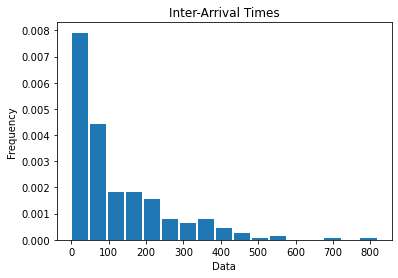
\includegraphics[width=\textwidth]{fig1.png}
        \caption{}
        \label{fig:img1}
    \end{subfigure}
    \hfill
    \begin{subfigure}[b]{0.45\textwidth}
        \centering
        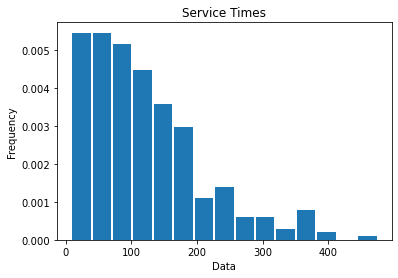
\includegraphics[width=\textwidth]{fig2.png}
        \caption{}
        \label{fig:img2}
    \end{subfigure}

    \caption{Histograms of inter-arrival times and service times}
    \label{fig:two-figs}
\end{figure}

Mauris rhoncus fringilla mollis. Ut tincidunt eros vel dolor aliquam, at consequat erat malesuada. Morbi interdum, lectus non dictum efficitur, mi erat molestie enim, quis gravida felis mi in arcu. Sed sit amet leo eget urna maximus sollicitudin sit amet et nisi. Donec maximus neque a tortor sagittis eleifend. Maecenas felis tortor, feugiat et ipsum in, congue imperdiet lectus. Aenean porta suscipit neque in rutrum. In eros erat, vulputate eu consequat vitae, facilisis nec felis.

\begin{figure}[h]
    \centering
    \begin{subfigure}[b]{0.45\textwidth}
        \centering
        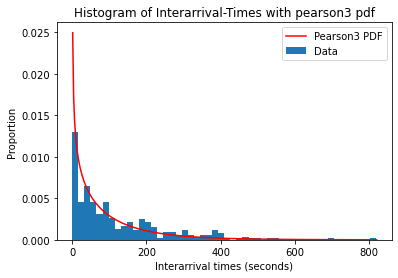
\includegraphics[width=\textwidth]{fig3.png}
        \caption{}
        \label{fig:img3}
    \end{subfigure}
    \hfill
    \begin{subfigure}[b]{0.45\textwidth}
        \centering
        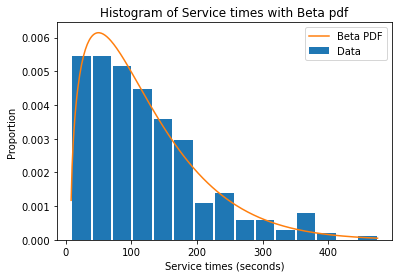
\includegraphics[width=\textwidth]{fig4.png}
        \caption{}
        \label{fig:img4}
    \end{subfigure}

    \caption{Histograms with best fit distribution pdf overlayed}
    \label{fig:two-figs2}
\end{figure}

Mauris rhoncus fringilla mollis. Ut tincidunt eros vel dolor aliquam, at consequat erat malesuada. Morbi interdum, lectus non dictum efficitur, mi erat molestie enim, quis gravida felis mi in arcu. Sed sit amet leo eget urna maximus sollicitudin sit amet et nisi. Donec maximus neque a tortor sagittis eleifend. Maecenas felis tortor, feugiat et ipsum in, congue imperdiet lectus. Aenean porta suscipit neque in rutrum. In eros erat, vulputate eu consequat vitae, facilisis nec felis.

Nullam dictum enim a diam finibus pretium. Nulla posuere mi vitae ultrices rutrum. Proin pellentesque neque id vulputate sollicitudin. Fusce malesuada dignissim dolor, non suscipit magna convallis semper. Vivamus turpis mauris, semper in quam quis, ultrices vulputate eros. Nulla finibus varius diam, vitae convallis lacus rutrum in. Pellentesque imperdiet gravida odio, hendrerit sagittis tellus sollicitudin id. Curabitur tincidunt ante mauris, eu venenatis tellus congue at.

\section{Simulation models}

\subsection{Performance Measures of collected data (Tama)}

\begin{table}[h!]
    \centering
    \caption{This is the caption that goes at the top of the table}
    \begin{tabu}{*{2}{X[c]}}
        \toprule
        \textbf{Performance Measures} & \textbf{Values calculated from data}\\
        \midrule
        Average time in system (seconds), $W$   & 140.07 \\
        Average number of customers in the system, $L$ & 1.1819\\
        Proportion of time servers are busy, $B$ & 0.61148  \\
        Effective arrival rate (per second), $\lambda_{\text{eff}}$ & 0.0084381\\
        \bottomrule
    \end{tabu}
    \label{tab:Original Data PF}
\end{table}

\begin{table}[h!]
    \centering
    \caption{This is the caption that goes at the top of the table}
    \begin{tabu}{*{2}{X[c]}}
        \toprule
        \textbf{Other parameters} & \textbf{Values calculated from data} \\
        \midrule
        Average Inter-arrival time $\frac{1}{\lambda}$ (seconds) & 120.329  \\
        Average Service time, $W_s$ (seconds) & 120.77  \\
        Average Queue Time, $W_q$ (seconds) & 19.295  \\
        \bottomrule
    \end{tabu}
    \label{tab:Original Data Other}
\end{table}



Suspendisse accumsan ante velit, a tempor urna porta ac. Proin porttitor, velit non rutrum tincidunt, nibh nulla mattis urna, vitae lobortis erat dui eget risus. Proin tincidunt tincidunt orci eget auctor. Mauris id sodales velit. Aliquam faucibus quam eu tellus varius, molestie dapibus risus sodales. Nullam feugiat vitae augue non ullamcorper. Nulla et nibh orci. Praesent lacus est, mollis efficitur ligula eget, condimentum tempus risus. Nullam auctor placerat dignissim.

\subsection{M1 model (Patrick)}

Suspendisse accumsan ante velit, a tempor urna porta ac. Proin porttitor, velit non rutrum tincidunt, nibh nulla mattis urna, vitae 

$$
\pi_{0} = \frac{1}{\sum_{k=0}^{s-1}{\frac{\rho^k}{k!}} + \frac{\rho^s}{s!}\frac{1}{1-\frac{\rho}{s}}}
$$

$$
\pi_{0} = \frac{1}{\frac{\rho^0}{0!} + \frac{\rho^1}{1!} + \frac{\rho^2}{2!} + \frac{\rho^3}{3!}\frac{1}{1-\frac{\rho}{3}}}
$$

$$
\pi_{0} = \frac{1}{1 + \rho + \frac{\rho^2}{2} + \frac{\rho^3}{6}\frac{1}{1-\frac{\rho}{3}}}
$$

$$
\pi_{0} = 0.3690202951
$$

$$
B = 1-\pi_{0} = 0.6309797049
$$

$$
L = \pi_{0}\frac{\frac{\rho^{s+1}}{s!s}}{(1-\frac{\rho}{s})^2}+\rho
$$

$$
L = \pi_{0}\frac{\frac{\rho^{4}}{3!3}}{(1-\frac{\rho}{3})^2}+\rho
$$

$$
L = 1.033745189
$$

$$
W = \frac{L}{\lambda} = 124.3899904
$$



Suspendisse accumsan ante velit, a tempor urna porta ac. Proin porttitor, velit non rutrum tincidunt, nibh nulla mattis urna, vitae lobortis erat dui eget risus. Proin tincidunt tincidunt orci eget auctor. Mauris id sodales velit. Aliquam faucibus quam eu tellus

\begin{table}[h!]
    \centering
    \caption{This is the caption that goes at the top of the table}
    \begin{tabu}{*{3}{X[c]}}
        \toprule
        \textbf{Performance Measures} & \textbf{Collected Data} & \textbf{M1 model}\\
        \midrule
        $W$ & 140.07 & 124.33\\
        $L$ & 1.1819 & 1.0435\\
        $B$ & 0.61148 & 0.63064\\
        $\lambda_{\text{eff}}$ & 0.0084381 & 0.0083952\\
        \bottomrule
    \end{tabu}
    \label{tab:M1}
\end{table}

Suspendisse accumsan ante velit, a tempor urna porta ac. Proin porttitor, velit non rutrum tincidunt, nibh nulla mattis urna, vitae lobortis erat dui eget risus. Proin tincidunt tincidunt orci eget auctor. Mauris id sodales velit. Aliquam faucibus quam eu tellus varius, molestie dapibus risus sodales. Nullam feugiat vitae augue non ullamcorper. Nulla et nibh orci. Praesent lacus est, mollis efficitur ligula eget, condimentum tempus risus. Nullam auctor placerat dignissim.

\subsection{M2 model (Vivian)}

In this model, the interarrival times is:\newline
pearson3(skew=2.43659632424228, loc=89.15123787553043, scale=108.61278925458328)\newline

The service times is\newline
beta(a=1.4923327932636143, b=15.801670930407775, loc=7.642594962182772, scale=1311.3920705953165).\newline

The performance simulated by this model is from the table below:

\begin{table}[H]
    \centering
    \caption{Best fit model}
    \begin{tabu}{*{3}{X[c]}}
        \toprule
        \textbf{Performance Measures} & \textbf{Collected Data} & \textbf{M2 model}\\
        \midrule
        $W$ & 140.07 & 143.28\\
        $L$ & 1.1819 & 1.6283\\
        $B$ & 0.61148 & 0.71400\\
        $\lambda_{\text{eff}}$ & 0.0084381 & 0.011347\\
        \bottomrule
    \end{tabu}
    \label{tab:M2}
\end{table}



\subsection{M3 model (Kevin)}

\begin{table}[h!]
    \centering
    \caption{This is the caption that goes at the top of the table}
    \begin{tabu}{*{3}{X[c]}}
        \toprule
        \textbf{Performance Measures} & \textbf{Collected Data} & \textbf{M3 model}\\
        \midrule
        $W$ & 140.07 & 127.14\\
        $L$ & 1.1819 & 1.0853\\
        $B$ & 0.61148 & 0.62465\\
        $\lambda_{\text{eff}}$ & 0.0084381 & 0.0085284\\
        \bottomrule
    \end{tabu}
    \label{tab:M3}
\end{table}


Suspendisse accumsan ante velit, a tempor urna porta ac. Proin porttitor, velit non rutrum tincidunt, nibh nulla mattis urna, vitae lobortis erat dui eget risus. Proin tincidunt tincidunt orci eget auctor. Mauris id sodales velit. Aliquam faucibus quam eu tellus varius, molestie dapibus risus sodales. Nullam feugiat vitae augue non ullamcorper. Nulla et nibh orci. Praesent lacus est, mollis efficitur ligula eget, condimentum tempus risus. Nullam auctor placerat dignissim.

\section{Conclusion}

Nullam dictum enim a diam finibus pretium. Nulla posuere mi vitae ultrices rutrum. Proin pellentesque neque id vulputate sollicitudin. Fusce malesuada dignissim dolor, non suscipit magna convallis semper. Vivamus turpis mauris, semper in quam quis, ultrices vulputate eros. Nulla finibus varius diam, vitae convallis lacus rutrum in. Pellentesque imperdiet gravida odio, hendrerit sagittis tellus sollicitudin id. Curabitur tincidunt ante mauris, eu venenatis tellus congue at.

Aenean non ante lacus. Proin fermentum sapien ut tempor mollis. Maecenas semper, sem cursus efficitur blandit, sapien felis varius massa, at ullamcorper neque libero vel elit. Donec scelerisque ipsum purus, in volutpat sapien facilisis eget. Proin nulla urna, ullamcorper eget urna eget, auctor pharetra mauris. Etiam quis ligula eget elit volutpat sollicitudin. In dolor tortor, iaculis et bibendum eget, gravida at nisl. Nunc tempus dolor in nisi hendrerit, eu fringilla nulla fringilla. Proin vel rutrum nisi, in gravida elit. Aliquam in erat sodales, sodales arcu luctus, laoreet metus. Integer vehicula odio ultricies faucibus bibendum. Curabitur fringilla a ipsum ut imperdiet. Mauris vulputate, lorem vel bibendum ultrices, ex enim vulputate nisi, a blandit urna quam in enim. Donec ac lacus sollicitudin, vulputate dui at, auctor velit. In hac habitasse platea dictumst. Nulla venenatis tellus sed mi rutrum, non auctor sem lacinia.

\end{document}
